% \begin{blocksection}

\question Draw the tree that is created by the following statement:

\begin{lstlisting}
tree('hello',
    [tree('how', []),
     tree('are',
        [tree('you', []),
         tree('doing', [])]),
     tree('from', []),
     tree('CSM',
        [tree('61A', [])])])
\end{lstlisting}
\begin{solution}
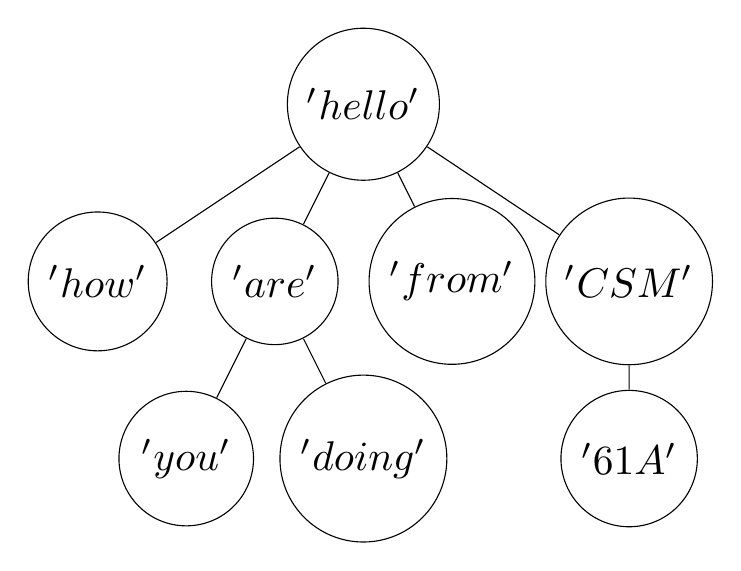
\begin{tikzpicture}[scale=1.5, transform shape]
    \node [circle, draw] (z) {$'hello'$}
        child {node [circle, draw] (a) {$'how'$}}
        child {node [circle, draw] (b) {$'are'$}
            child {node [circle, draw] (e) {$'you'$}}
            child {node [circle, draw] (f) {$'doing'$}}
        }
        child {node [circle, draw] (c) {$'from'$}}
        child {node [circle, draw] (d) {$'CSM'$}
            child {node [circle, draw] (g) {$'61A'$}}
        };
\end{tikzpicture}
\end{solution}

% \end{blocksection}